\documentclass[10pt,aspectratio=169]{beamer}
\setbeamertemplate{navigation symbols}{}
\usepackage[T1]{fontenc}
\usepackage{lmodern}
\usepackage{amsmath,amssymb,booktabs,array,tikz,colortbl,xspace}
\usetikzlibrary{positioning,arrows.meta,calc,fit}
\usetheme{MIT}
\graphicspath{{../results/figures/}}

\definecolor{ink}{HTML}{1F2933}
\definecolor{muted}{HTML}{616E7C}
\definecolor{accent}{HTML}{A31F34}
\definecolor{markblue}{HTML}{1F4E79}
\definecolor{soft}{HTML}{E8EDF2}
\definecolor{pool}{HTML}{2A78D6}
\definecolor{rnn}{HTML}{EB6834}
\setbeamercolor{normal text}{fg=ink}
\setbeamerfont{frametitle}{size=\normalsize,series=\bfseries}
\setlength{\tabcolsep}{4pt}
\renewcommand{\arraystretch}{1.05}
\setlength{\fboxsep}{1.5pt}

\newcommand{\hd}[1]{{\footnotesize\bfseries\color{accent}#1}\par\vspace{2pt}}
\newcommand{\best}[1]{\cellcolor{soft}\textbf{#1}}
\newcommand{\src}[1]{\vfill\vspace{5pt}{\fontsize{6.5}{7.5}\selectfont\color{muted}#1\par}\vspace{1pt}}
\newcommand{\tk}[1]{\fcolorbox{muted!50}{white}{\strut\texttt{#1}}}
\newcommand{\tkn}[1]{\fcolorbox{accent}{white}{\strut\textcolor{accent}{\texttt{\textbf{#1}}}}}
\newcommand{\pp}{\,pp\xspace}
\newcommand{\sd}[1]{{\color{muted}\fontsize{5.5}{6}\selectfont\,$\pm$#1}}

\author[Alcocer, Bhathawala, Jayasimha]{Alcocer, Bhathawala, Jayasimha}
\title[NLP1 Project 2: MNLI]{NLP1 Project 2}

\begin{document}

%%%%%%%%%%%%%%%%%%%%%%%%%%%%%%%%%%%%%%%%%%%%%%%%%%%%%%%%%%%%%%%%
\begin{frame}[t]{Q1 Table: 300d vectors read with the tokens they were trained on}
\vspace{-4pt}
\begin{columns}[T,onlytextwidth]
\begin{column}{.50\textwidth}
\hd{Frozen tables (tuning accuracy \%, $\pm$ SD of 3 seeds)}
{\scriptsize\centering\setlength{\tabcolsep}{3pt}
\begin{tabular}{@{}lrrr@{}}\toprule
Table & coverage & pool & BiLSTM\\\midrule
GloVe 2024 50d (tutorial 2) & 99.3 & 49.9\sd{0.3} & --\\
GloVe 6B 50d & 99.3 & 49.6\sd{0.1} & --\\
GloVe 6B 300d & 99.3 & 58.0\sd{0.1} & 70.7\sd{0.1}\\
GloVe 840B (Common Crawl) & 99.6 & 59.6\sd{0.2} & 71.6\sd{0.1}\\
word2vec, Google News & 88.1 & 59.3\sd{0.2} & 71.7\sd{0.1}\\
counter-fitted & 85.7 & 60.4\sd{0.1} & 71.3\sd{0.3}\\
fastText crawl & 98.9 & 60.8\sd{0.7} & 72.5\sd{0.2}\\
ConceptNet Numberbatch & 87.1 & \best{61.3}\sd{0.3} & \best{73.0}\sd{0.4}\\\midrule
scratch: 300d, trained & own vocab. & 63.1\sd{0.2} & 67.2\sd{0.1}\\\bottomrule
\end{tabular}\par}
\vspace{4pt}
{\scriptsize 50\,$\to$\,300d: $+8.4$\pp. Numberbatch is best for both encoders, but for pool within
seed noise of fastText; fine-tuned, pool prefers fastText (Q3). Frozen pool underfits, so a trained
scratch table beats every frozen one; the BiLSTM does better with a frozen table.\par}
\end{column}
\begin{column}{.47\textwidth}
\hd{Coherent tokens: the table's own strings}
{\scriptsize
\vspace{2pt}\tk{You}\tk{do}\tk{n't}\tk{know}\par\vspace{2pt}
NLTK = MNLI parse leaves = GloVe 840B's training tokens.\par\vspace{2pt}
fastText has no \tkn{n't}, so 37,814 negations would get the unknown vector. Our \texttt{nltk-not} spells it out:\par\vspace{2pt}
\tk{do}\tkn{not}\ \ \tk{can}\tkn{not}\ \ \tk{will}\tkn{not}\par\vspace{2pt}
Coverage 98.89\,$\to$\,99.47\%. In fine-tuned pool, fastText gains $+0.46$\pp (SD 0.09) with
\texttt{nltk-not} but $-0.18$\pp with plain NLTK: our final pool model.\par}
\vspace{3pt}
\hd{Incoherent tokens cost accuracy ($\Delta$ to NLTK, pp)}
{\scriptsize\centering
\begin{tabular}{@{}lrr@{}}\toprule
Tokeniser & GloVe 840B & fastText\\\midrule
NLTK Treebank (reference: accuracy) & 59.6\sd{0.2} & 60.8\sd{0.7}\\\midrule
MNLI parse leaves & $-0.1$\sd{0.2} & $-0.2$\sd{0.2}\\
whitespace (\tk{dog.} $\neq$ \tk{dog}) & $-2.4$\sd{0.3} & $-1.4$\sd{1.2}\\
tutorial 2 BoW (no \emph{not, all}) & $-5.4$\sd{0.7} & $-5.2$\sd{0.7}\\\bottomrule
\end{tabular}\par}
\end{column}
\end{columns}
\src{Code: \href{https://github.com/miguelalcocker/nlp1-student-group01/tree/main/project2}{github.com/miguelalcocker/nlp1-student-group01/tree/main/project2}. AI use: \texttt{project2/AI\_USE.md}.
Tuning set, $\pm$ SD of 3 seeds ($\Delta$: seed-paired). Coverage: running tokens with a vector; scratch: own vocabulary (types seen $\ge$\,2$\times$).}
\end{frame}

%%%%%%%%%%%%%%%%%%%%%%%%%%%%%%%%%%%%%%%%%%%%%%%%%%%%%%%%%%%%%%%%
\begin{frame}[t]{Q2 What the tables capture: relatedness, so antonyms sit close}
\vspace{-4pt}
\begin{columns}[T,onlytextwidth]
\begin{column}{.52\textwidth}
\hd{WordNet relations among 10,649 MNLI words (cosine)}
{\scriptsize\centering
\begin{tabular}{@{}lrrrr@{}}\toprule
Table & synonym & antonym & AUC syn$>$ant & AUC E$>$N\\\midrule
GloVe 840B & 0.40 & 0.55 & 0.27 & 0.600\\
fastText & 0.32 & 0.52 & 0.23 & 0.627\\
word2vec & 0.27 & 0.42 & 0.28 & 0.614\\
counter-fitted & 0.39 & \best{$-$0.02} & \best{0.96} & 0.640\\
Numberbatch & 0.34 & 0.44 & 0.35 & \best{0.652}\\\bottomrule
\end{tabular}\par}
\vspace{2pt}
{\scriptsize AUC syn$>$ant: chance a synonym pair is closer than an antonym pair (0.5 = no separation).
AUC E$>$N: task evidence; for each pair, mean best cosine of new hypothesis words with the premise,
entailment vs neutral. Numberbatch aligns best and wins in accuracy (Q1).\par}
\vspace{6pt}
\hd{Nearest neighbours in GloVe 840B}
{\scriptsize \emph{always} $\to$ \textbf{never}, really, definitely \quad
\emph{increase} $\to$ increased, \textbf{decrease} \quad
\emph{none} $\to$ neither, nothing\par}
\end{column}
\begin{column}{.45\textwidth}
\hd{Why it is troubling for NLI}
{\scriptsize
2.9\% of training pairs contain a WordNet antonym pair across premise and hypothesis;
\textbf{64.6\% of them are contradictions}. GloVe 840B gives that pair a cosine of 0.66.\\[3pt]
Counter-fitting fixes the geometry, but not accuracy: frozen pool $+0.8$\pp, BiLSTM $-0.3$\pp
(it covers 85.7\% of tokens).\par}
\vspace{6pt}
\hd{Other limitations we checked}
{\scriptsize
\begin{itemize}\setlength{\itemsep}{1pt}
\item One vector per type: \emph{right} $\to$ way, you, sure, wrong.
\item Gender direction (he$-$she), all four tables: \emph{nurse, secretary} vs \emph{engineer, architect}.
\item No order: \emph{A dog bit a man} = \emph{A man bit a dog} after pooling.
\end{itemize}\par}
\vspace{2pt}
\hd{Does it show in the errors? (Q6)}
{\scriptsize Pairs with an antonym pair: BiLSTM 70.8\%, pool 61.3\%, P1 58.9\%.\par}
\end{column}
\end{columns}
\src{Words: seen 20+ times in MNLI and covered by every table; synonym and antonym pairs from WordNet. AUC E$>$N on 30,000 training pairs, entailment vs neutral.}
\end{frame}

%%%%%%%%%%%%%%%%%%%%%%%%%%%%%%%%%%%%%%%%%%%%%%%%%%%%%%%%%%%%%%%%
\begin{frame}[t]{Q3 Embed-and-pool: fine-tune the table; it ties project 1, not beats it}
\vspace{-4pt}
\begin{columns}[T,onlytextwidth]
\begin{column}{.56\textwidth}
\hd{One change at a time, then again around the new base}
\includegraphics[width=\linewidth]{q3_pool_search.pdf}
\end{column}
\begin{column}{.41\textwidth}
\hd{Why fine-tuning wins}
{\scriptsize
Frozen tables underfit (train $\approx$ tuning $\approx$ 60\%), so capacity helps most: fine-tuning
$+5.1$, 512d projection $+3.9$, both $+5.8$\pp, the step-2 base. Around it nothing moves
$>0.5$\pp but a scratch table ($-2.3$).\par}
\vspace{6pt}
\hd{Better than last week? (CV)}
{\scriptsize\centering
\begin{tabular}{@{}lr@{}}\toprule
System & accuracy\\\midrule
pool, fine-tuned fastText & \best{65.17}\sd{0.21}\\
P1: BPE + overlap, Siamese & 64.85\sd{0.21}\\
pool, scratch table & 62.24\sd{0.29}\\
pool, hypothesis only & 54.42\sd{0.19}\\\bottomrule
\end{tabular}\par}
\vspace{3pt}
{\scriptsize No: pool $-$ P1 $= +0.3$\pp, \textbf{P(tie) = 1.00}. P1 pooled scratch BPE vectors
plus overlap features; pretrained vectors match it without them, and adding overlap does not help
($-0.4$\pp). Pretraining: $+2.9$\pp (P = 1.00).\par}
\end{column}
\end{columns}
\src{Left: tuning set, 3 seeds; dot: mean $\Delta$ to the base, paired by seed; bar: SD of that $\Delta$ over seeds (in step 1 mostly hidden by the dot); grey band $\pm$1\pp.
Step 1 base: frozen GloVe 840B; step 2 base: fine-tuned + 512d projection. Final: fine-tuned fastText, \texttt{nltk-not}, 512d projection, mean pooling, MLP 512. CV: 5 folds $\times$ 3, $\pm$ SD over the 15 scores.}
\end{frame}

%%%%%%%%%%%%%%%%%%%%%%%%%%%%%%%%%%%%%%%%%%%%%%%%%%%%%%%%%%%%%%%%
\begin{frame}[t]{Q4 Recurrent encoder: BiLSTM-max on frozen Numberbatch, +7.2\,pp over pooling}
\vspace{-4pt}
\begin{columns}[T,onlytextwidth]
\begin{column}{.55\textwidth}
\hd{Data size: 1--100\% of the premises (fold 0, 3 repetitions)}
\includegraphics[width=\linewidth]{q4_datasize.pdf}
\vspace{2pt}
{\scriptsize Pretraining helps at every size, and more for the BiLSTM ($+6$ to $+8$\pp, most at 1\%: $+8.1$)
than for pool ($+3$ to $+4$\pp). The gain does not vanish with 280k pairs, and all four curves still
rise linearly in log(data): more data would help every model.\par}
\end{column}
\begin{column}{.42\textwidth}
\hd{Design: the sequence summary matters most}
{\scriptsize
Max over states beats mean ($-2.0$) and last state ($-2.5$), as in InferSent; Numberbatch $+1.4$.
Size, depth, cell, direction, decay: $<1$\pp each; tutorial 2's LSTM $-6.3$\pp. Choices: Q5.\par}
\vspace{5pt}
\hd{Over-fitting: yes, so keep the table frozen}
{\scriptsize Train 80.7\% vs CV 72.4\%. Fine-tuning adds 27M parameters to 2.2M: $-1.5$\pp.
Limited by early stopping, dropout, word dropout, decay 0.1.\par}
\vspace{5pt}
\hd{How far does it go? (CV)}
{\scriptsize\centering
\begin{tabular}{@{}lrr@{}}\toprule
 & BiLSTM & pool\\\midrule
pretrained & \best{72.41}\sd{0.21} & 65.17\sd{0.21}\\
scratch table & 66.35\sd{0.26} & 62.24\sd{0.29}\\
hypothesis only & 56.95\sd{0.26} & 54.42\sd{0.19}\\\bottomrule
\end{tabular}\par}
\vspace{2pt}
{\scriptsize BiLSTM $-$ pool $+7.2$\pp, $-$ P1 $+7.6$\pp (P = 1.00); with scratch tables still $+4.1$\pp.
Matched / mismatched validation: 71.9 / 72.9\%.\par}
\end{column}
\end{columns}
\src{Data size: accuracy on held-out fold 0; bars: SD over 3 repetitions (left: mostly hidden by the markers; right: SD of the seed-paired gain).
Design: tuning set, $\Delta$ to the base paired by seed. CV: 5 folds $\times$ 3, $\pm$ SD over the 15 scores. No final or data-size fit hit the 60-epoch cap.}
\end{frame}

%%%%%%%%%%%%%%%%%%%%%%%%%%%%%%%%%%%%%%%%%%%%%%%%%%%%%%%%%%%%%%%%
\begin{frame}[t]{Q5 Decisions under uncertainty: 3 seeds per setting, paired differences, CV last}
\vspace{-4pt}
\begin{columns}[T,onlytextwidth]
\begin{column}{.52\textwidth}
\hd{Search: one change at a time, twice}
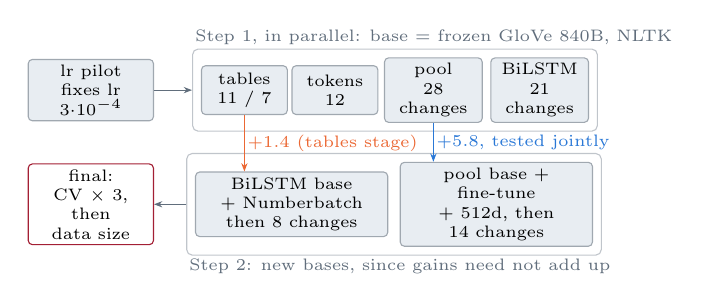
\begin{tikzpicture}[font=\fontsize{6}{7}\selectfont,>={Stealth[length=3pt]},
  ch/.style={draw=muted!60,rounded corners=1.5pt,fill=soft,inner sep=2pt,align=center,minimum height=.62cm},
  box/.style={draw=muted!40,rounded corners=2pt,inner sep=3pt},
  lab/.style={anchor=south west,inner sep=1pt,text=muted},
  fin/.style={ch,fill=white,draw=accent}]
\node[ch,text width=1.45cm] (lr) at (0,0) {lr pilot\\fixes lr $3{\cdot}10^{-4}$};
\node[ch,text width=0.95cm] (tab) at (1.95,0) {tables\\11 / 7};
\node[ch,text width=0.95cm] (tok) at (3.1,0) {tokens\\12};
\node[ch,text width=1.1cm] (p1) at (4.35,0) {pool\\28 changes};
\node[ch,text width=1.1cm] (r1) at (5.7,0) {BiLSTM\\21 changes};
\node[box,fit=(tab)(r1)] (s1) {};
\node[lab] at (s1.north west) {Step 1, in parallel: base = frozen GloVe 840B, NLTK};
\node[ch,text width=2.3cm] (r2) at (2.55,-1.45) {BiLSTM base + Numberbatch\\then 8 changes};
\node[ch,text width=2.3cm] (p2) at (5.15,-1.45) {pool base + fine-tune\\+ 512d, then 14 changes};
\node[box,fit=(r2)(p2)] (s2) {};
\node[lab,anchor=north west] at (s2.south west) {Step 2: new bases, since gains need not add up};
\node[fin,text width=1.45cm] (cv) at (0,-1.45) {final: CV $\times$ 3,\\then data size};
\draw[->,muted] (lr)--(s1.west|-lr);
\draw[->,pool] (p1.south)--node[right,pos=.5,inner sep=1pt]{$+5.8$, tested jointly} (p1.south|-p2.north);
\draw[->,rnn] (tab.south)--node[right,pos=.5,inner sep=1pt]{$+1.4$ (tables stage)} (tab.south|-r2.north);
\draw[->,muted] (s2.west)--(cv.east);
\end{tikzpicture}\par
\vspace{4pt}
\hd{Close calls in step 2 (BiLSTM, $\Delta$ to its base, 72.96\%)}
{\scriptsize\centering
\begin{tabular}{@{}lrl@{}}\toprule
Change & $\Delta$ (SD) & decision\\\midrule
decay 0.1 & $+0.35$ (0.42) & \best{kept}: step 1 $+0.71$\\
decay 0.1, 512 units, 2 layers & $+0.46$ (0.30) & tie, over-fits more\\
GRU instead of LSTM & $+0.03$ (0.27) & no gain\\\bottomrule
\end{tabular}\par}
\end{column}
\begin{column}{.45\textwidth}
\hd{Three things that would have misled us}
{\scriptsize
\textbf{Epoch cap.} A first run stopped at 20 epochs while BiLSTMs still improved: 51 fits set aside,
cap 60, and each fit records whether it hit it (1 of 462, a setting not chosen).\\[2pt]
\textbf{Learning rate $\times$ decay.} In AdamW the shrinkage per step is lr $\times$ wd: higher lr
lowered \emph{training} accuracy too, so the grid varies both.\\[2pt]
\textbf{Table scale.} Unit-norm tables are 7$\times$ smaller: at that scale counter-fitted and Numberbatch lose 1.6--1.7\pp, so all tables are rescaled to coordinate SD 0.4.\par}
\vspace{5pt}
\hd{Learning-rate pilot, before any search}
{\scriptsize\centering
\begin{tabular}{@{}lrr@{}}\toprule
lr & BiLSTM & pool\\\midrule
$3\cdot10^{-4}$ & \best{71.6}\sd{0.1} & \best{59.6}\sd{0.2}\\
$10^{-3}$ & 70.4\sd{0.4} & 57.8\sd{0.1}\\
$2\cdot10^{-3}$ / $3\cdot10^{-3}$ & 68.8\sd{0.2} & 56.3\sd{0.1}\\\bottomrule
\end{tabular}\par}
\vspace{2pt}
{\scriptsize It sets the centre, not a bound: steps 1 and 2 still test lr$/3$ and lr$\times3$.\par}
\end{column}
\end{columns}
\src{Every setting: 3 seeds; $\Delta$ to its base paired by seed (median seed SD 0.17\pp, max 0.74); close calls: SD of the paired $\Delta$.
Final comparisons: Bayesian correlated $t$-test on the 15 CV fold scores (runs = 3), ROPE $\pm$1\pp.}
\end{frame}

%%%%%%%%%%%%%%%%%%%%%%%%%%%%%%%%%%%%%%%%%%%%%%%%%%%%%%%%%%%%%%%%
\begin{frame}[t]{Q6 Error analysis: pretrained tables rely less on surface cues; neutral pairs remain hard}
\vspace{-4pt}
\begin{columns}[T,onlytextwidth]
\begin{column}{.47\textwidth}
\hd{What predicts a correct fit (19,647 val. pairs)}
\includegraphics[width=.86\linewidth]{q6_weights.pdf}
\vspace{2pt}
\hd{Features we tested (17, standardised)}
{\scriptsize Length, parse depth; overlap, alignment; negation, quantifiers, antonyms;
rarest word, words without vector; hypothesis-only BiLSTM's correctness and confidence
(model-specific); genre shift; gold label.\par}
\end{column}
\begin{column}{.50\textwidth}
\hd{Differences between designs (95\% interval excludes 0)}
{\scriptsize
\begin{itemize}\setlength{\itemsep}{1pt}
\item \textbf{Pretrained vs scratch}, both encoders: less weight on overlap, negation cue and
rare words ($-0.05$ each).
\item \textbf{BPE vs word tables}: tokens without a vector hurt pool and BiLSTM, not P1.
\item \textbf{Antonym pairs} (Q2) hurt P1, pool and scratch tables, not the BiLSTM (+0.03 vs pool).
\item \textbf{Long premises}, against our expectation, hurt the BiLSTM as much as pool
(parse depth: $-0.04$ vs pool); $>$30 tokens: 68.6\% vs 72.4\% overall.
\item \textbf{Artefacts}: hypothesis-only correctness predicts every design most ($+0.75$ to $+1.04$);
pairs it fails: BiLSTM 52.2\%, P1 46.3\%, pool 45.0\%.
\item \textbf{Neutral}: BiLSTM $-$ P1 is $+10.1$ (E), $+8.8$ (C), only $+3.8$\pp (N).
\end{itemize}\par}
\vspace{-1pt}
\hd{What we would prioritise}
{\scriptsize 1. Cross-sentence attention (ESIM-style): we compare sentences only after pooling,
which hurts neutral pairs and long premises. 2. Report the artefact-hard subset.
3. Subword vectors for missing words.\par}
\end{column}
\end{columns}
\src{Tutorial 2's Bayesian regression of correctness on standardised features, Binomial over the 15 CV fits of each pair; 4 chains, $\hat r \le 1.003$, 0 divergences.
The hypothesis-only model is a BiLSTM, which may favour the BiLSTM's weight on it.}
\end{frame}

\end{document}
